\chapter{Konzeption}
\label{Konzeption}
Nachfolgend wird die Konzeption des Projekts beschrieben. 
De Kommunikation wird nachrichtenbasiert umgesetzt. Dies bedeutet, dass die Komponenten des verteilten Systems kommunizieren, indem sie sich Nachrichten übermitteln können. Die Steuerung der Kommunikation wird primär von den als Master 
(siehe \ref{glossar}) ausgewählten Komponenten umgesetzt. Als Provider wird ein angepasster Webserver eingesetzt, die Verbindung der einzelnen Komponenten zueinander geschieht über WebSockets. Der Webserver basiert auf dem Javascript-Framework Node.js. \\


\section{Brute Force-Algorithmus}
\label{ideeBruteForce}
Grundlegend ist das Ziel des Projektes das Entschlüsseln eines vorgegebenen Passwortes. Das zu entschlüsselnde Passwort wird vor der Berechnung vom Benutzer eingetragen. Das eingetragene Passwort wird dann durch eine Hashfunktion geleitet. Der entstandene Hash wird gespeichert und dient als Zielbedingung der folgenden Berechnung. \\
Nun beginnt der eigentliche Angriff. Zu Beginn wird eine sogenannte \enquote{Dictionary-Attack} vorgenommen. Dies bedeutet, dass ein Wörterbuch mit häufig genutzten Passwörtern als Basis des Angriffs genutzt wird. Durch die vorangestellte Attacke auf Basis von häufig benutzten Passwörtern wird die Wahrscheinlichkeit, das gesuchte Passwort effizient zu identifizieren, deutlich erhöht. Der folgende Auszug aus der Passwortliste (des Dictionary) verdeutlicht das Prinzip dieser Angriffsmethode. \\
\texttt{Dictionary:}
\begin{lstlisting}[basicstyle=\ttfamily,numbers=left,numberstyle=\footnotesize\ttfamily,backgroundcolor=\color{sourcegray}]
	LOVE123
	LOVEME1
	Lamont1
	Leasowes2
	Lemon123
	Liberty
	Lindsay
	Lizard
	Love21
	MASTER
	MORIAH07
	MOSS18
	Madeline
	Margaret
	Master
	Matthew
	Maxwell
	Mellon
	Merlot
	Metallic
	Michael
\end{lstlisting}



Bleibt die Dictionary-Attack erfolglos, werden alle möglichen Zeichenkombinationen untersucht. \\
Die erste Idee war es, dass der steuernde Rechner alle möglichen Passwörter in einem Array ablegen wird. Das Muster der möglichen Passwörter sollte wie folgt aufgebaut werden: 
\texttt{Muster der zu berechnenden Passwörter:}
\begin{lstlisting}[basicstyle=\ttfamily,numbers=left,numberstyle=\footnotesize\ttfamily,backgroundcolor=\color{sourcegray}]
	Array passwordsUPPER = 
		[A*****,
	 	B*****,
	 	C*****,
	 	D*****,
	 	...
	]
	
	
	Array passwordsLOWER = 
		[a*****,
	 	b*****,
	 	c*****,
	 	d*****,
		...
	]
	
	

	Array passwordsNUM = 
		[1*****,
	 	2*****,
	 	3*****,
	 	4*****,
		...
	]
\end{lstlisting}

Die exemplarische Darstellung soll die geplante Aufteilung verdeutlichen. Die hier dargestellte feste Länge der Passwörter auf 6 Zeichen dient als Beispiel. In der Praxis werden alle möglichen Passwörter probiert, begonnen mit Passwörtern der Länge = 1. Wird kein Passwort ermittelt, so werden Passwörter der Länge n+1 erzeugt.  \\

\begin{figure}[!ht]
	\centering
		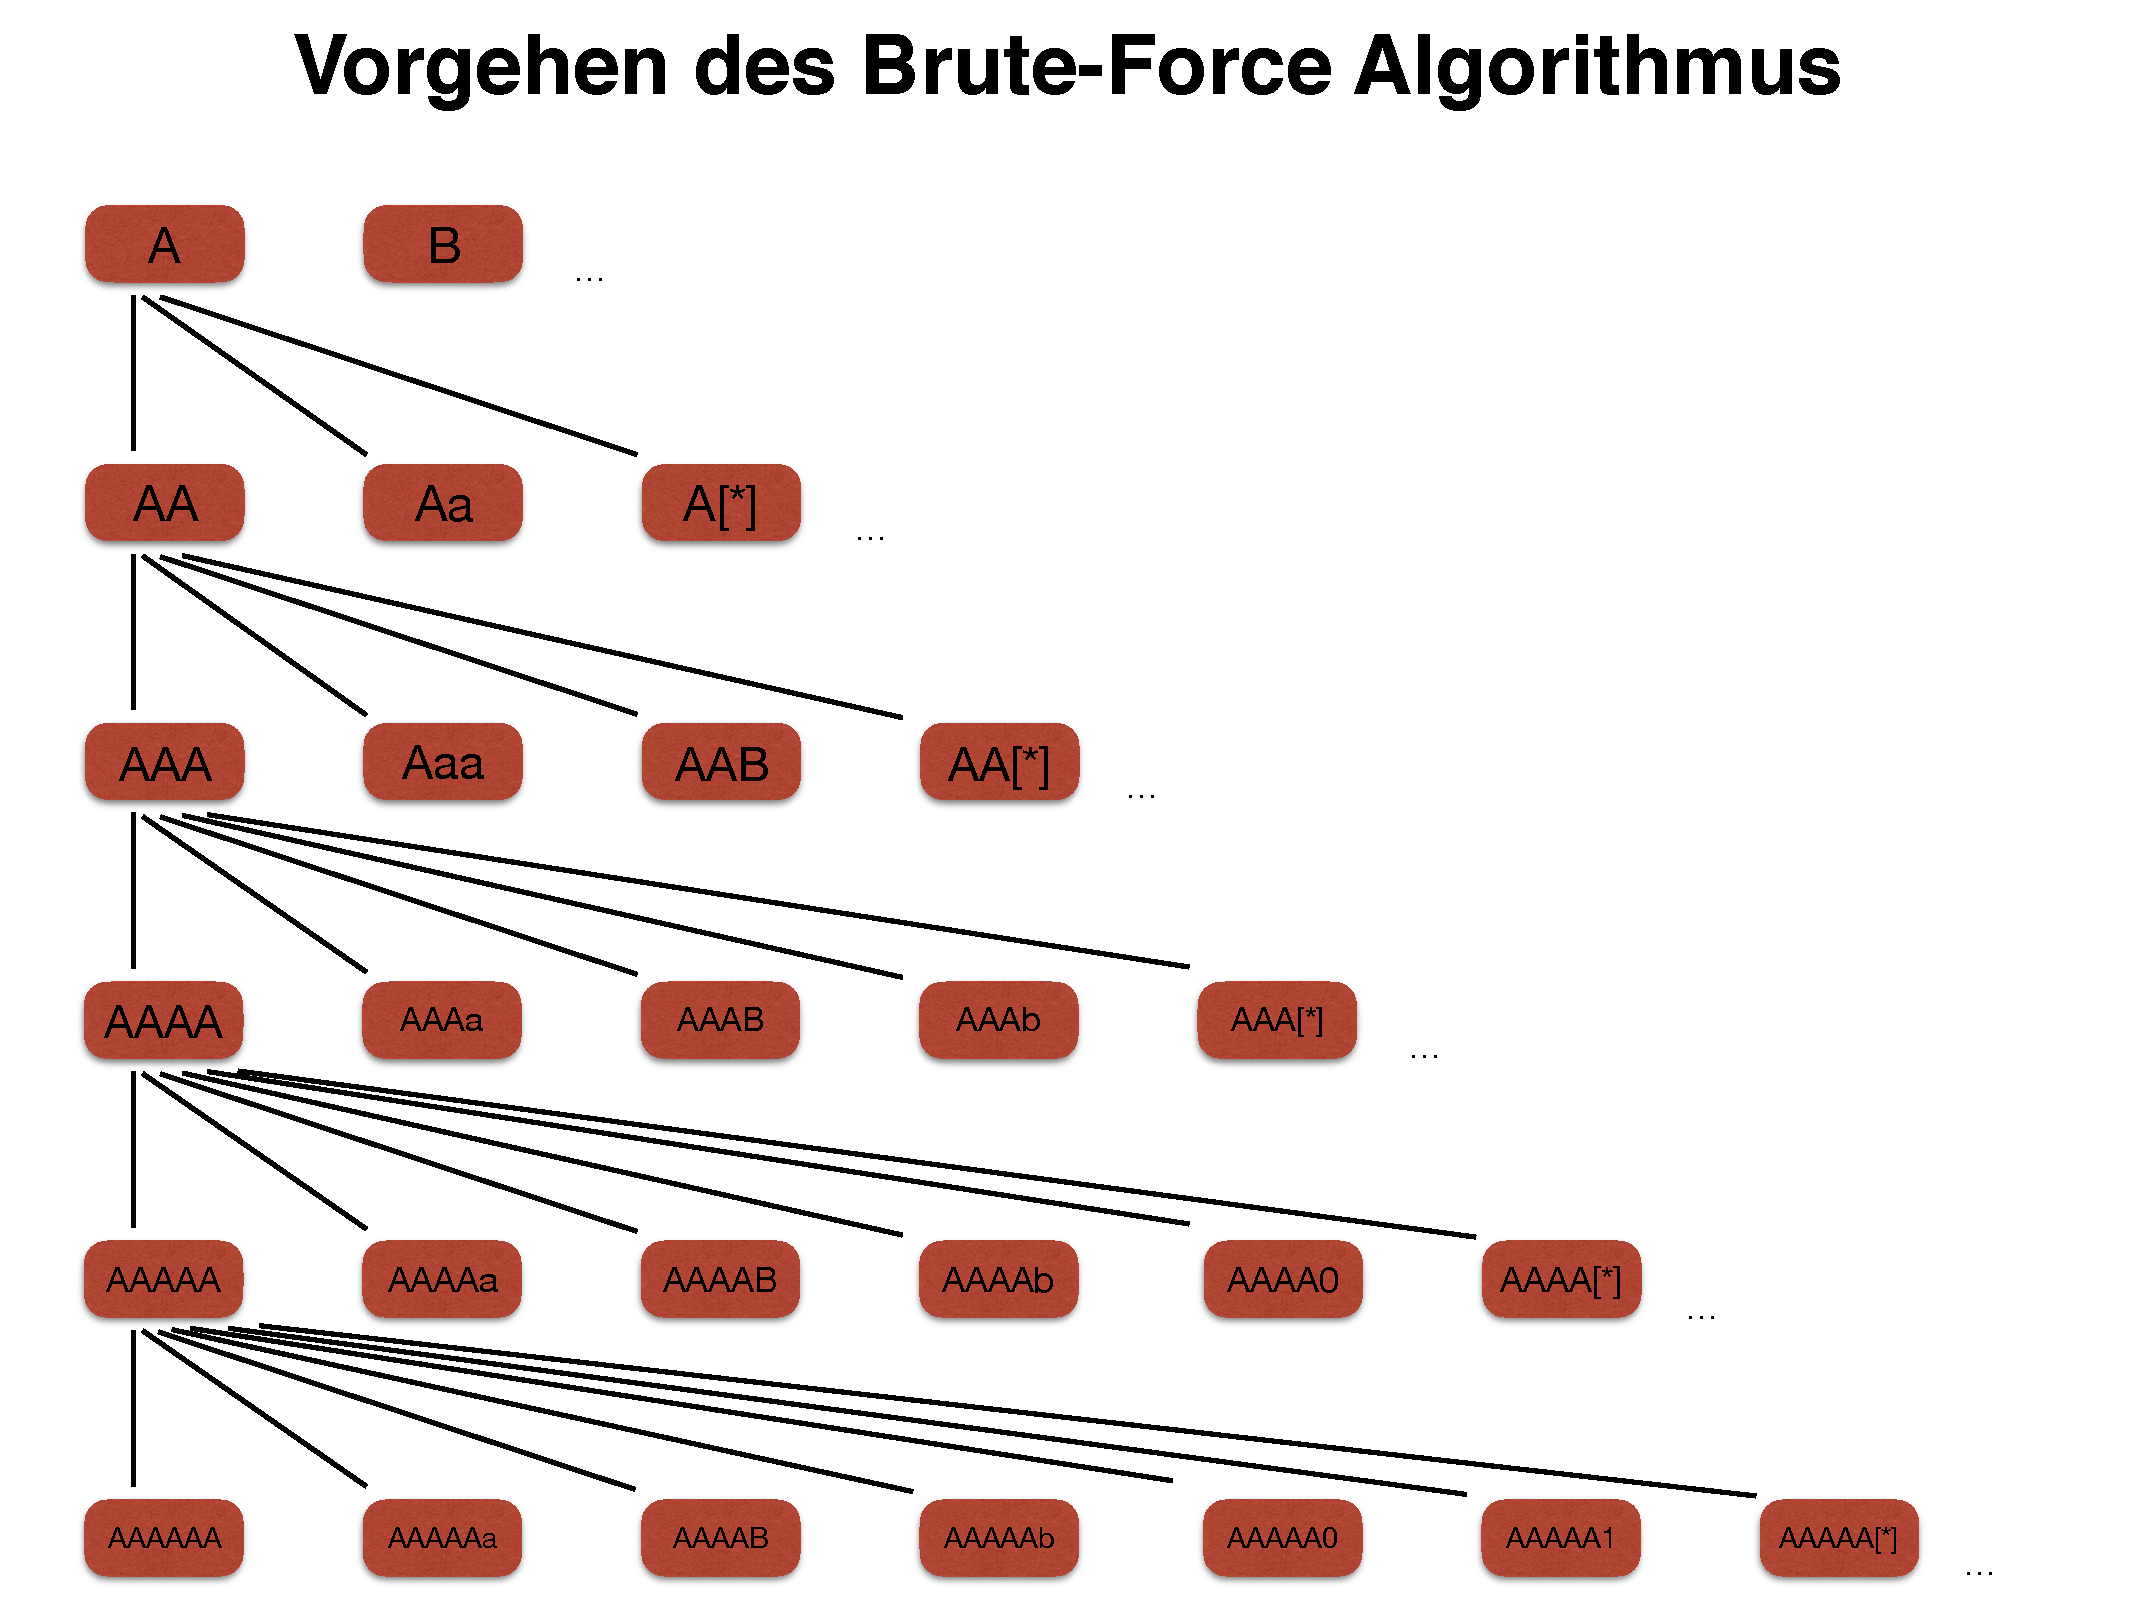
\includegraphics[natwidth=1200pt, natheight=349pt, width=1.0\textwidth]{images/SchaubildAlgorithmBreitensuche.pdf}
	\caption{Darstellung der Suchstrategie, die der Brute-Force Algorithmus zum Ermitteln des Passwortes benutzt.}
	\label{fig:showcase}
\end{figure}

